\section{Vocabulario de CicloCarriles}

Para el vocabulario asociado con los ciclocarriles para ciclistas se han obtenido los datos del portal de datos abiertos del ayuntamiento de Madrid \cite{datosMadrid_ciclocarriles}, en el cual se muestran las calles que disponen de ciclocarriles y alguna de sus características.
\newline
\newline
La organización del conjunto de datos se hará siguiendo el diagrama \ref{fig:diagramaOntologCicloCarr}

\begin{figure}[h]
	\centering
		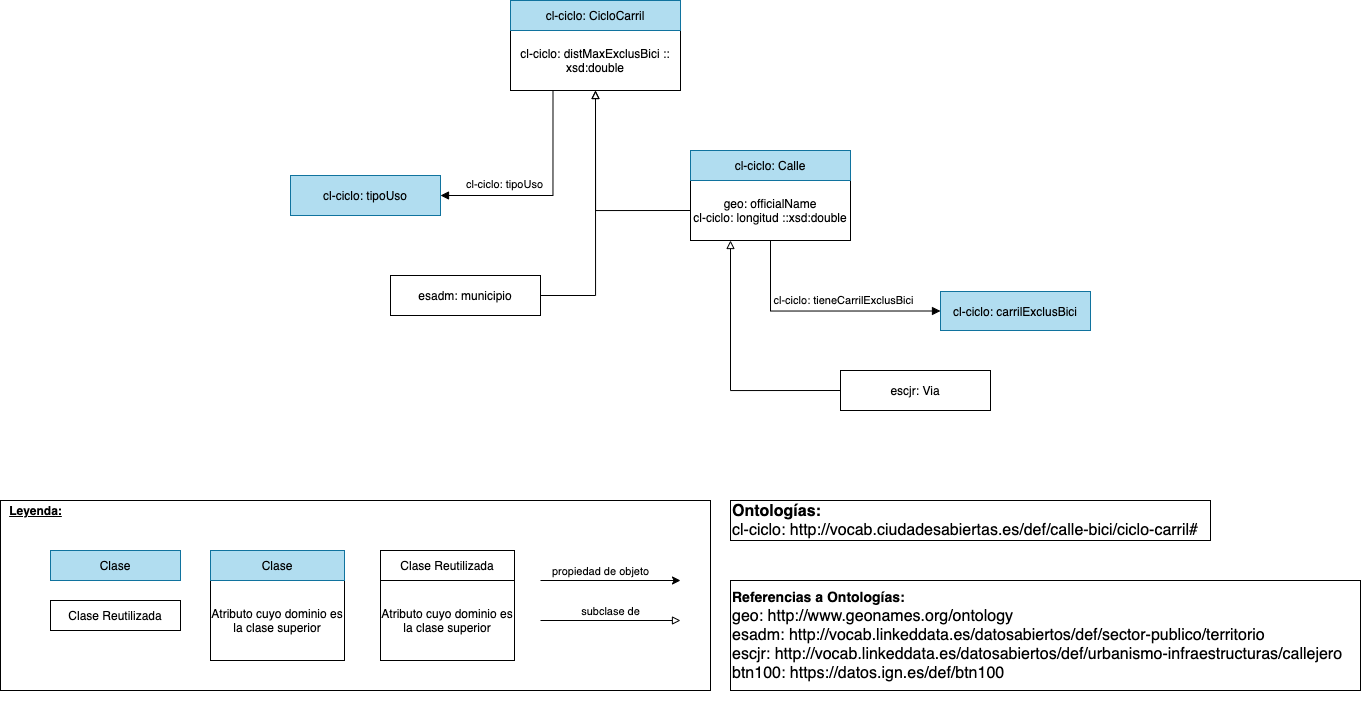
\includegraphics[angle=0, width=0.8\textwidth]{images/diagramaCicloCarril.png}  
	\caption{Diagrama de Ontología de ciclocarriles en Madrid.}
	\label{fig:diagramaOntologCicloCarr}
\end{figure}





Para la representación de los datos de ciclocarriles para ciclistas se han definido varias clases y propiedades. Se han reutilizado elementos ya definidos en el vocabulario de Callejero de ciudadesabiertas.es \cite{ciudadesbiertas_callejero}.
Se han añadido elementos como el identificador de via y el municipio (que siempre será Madrid).
El identificador de via se añadirá para cada caso a partir del nombre. Para ello se hará una reducción del nombre de la via a palabras clave, proceso detallado en la sección de Transformaciones de Vocabularios, y se cruzará con el dataset del callejero de Madrid \cite{datosmadrid_callejero}.
Se ha optado por omitir la propiedad "MinSimpTol" debido a que no aporta valor al conjunto al tener solo 2 valores, 0 para calles sin carril bici y 0.20 para calles que si disponen de él, información que puede inferirse del campo "MaxSimpTol" (renombrada "distMaxExclusBici"), con valor 0 para el primer caso y valor distinto de 0 para el segundo. Para representar esto se ha añadido la propiedad “carrilExclusBici” con valor booleano indicando si dispone de ese carril exclusivo o no.
La fecha proporcionada por el ayuntamiento se ha omitido debido a que no se sabe con exactitud su significado. En caso de que fuese fecha de creación del ciclocarril se debería añadir en futuras actualizaciones del vocabulario, sin embargo al ser en todos los registros la misma cabe la posibilidad de que sea la fecha de inserción en el dataset, lo cual no aporta información relevante y podría inducir a errores.
Para este caso el valor de "tipoUso" será siempre CICLOCARRIL.
Se han transformado los valores del campo longitud a metros (expresados en kilómetros en los datos de origen) para poder reutilizarlos con más facilidad.


\newpage
En la siguiente tabla se muestran los Namespaces usados.

\begin{figure}[h]
	\centering
		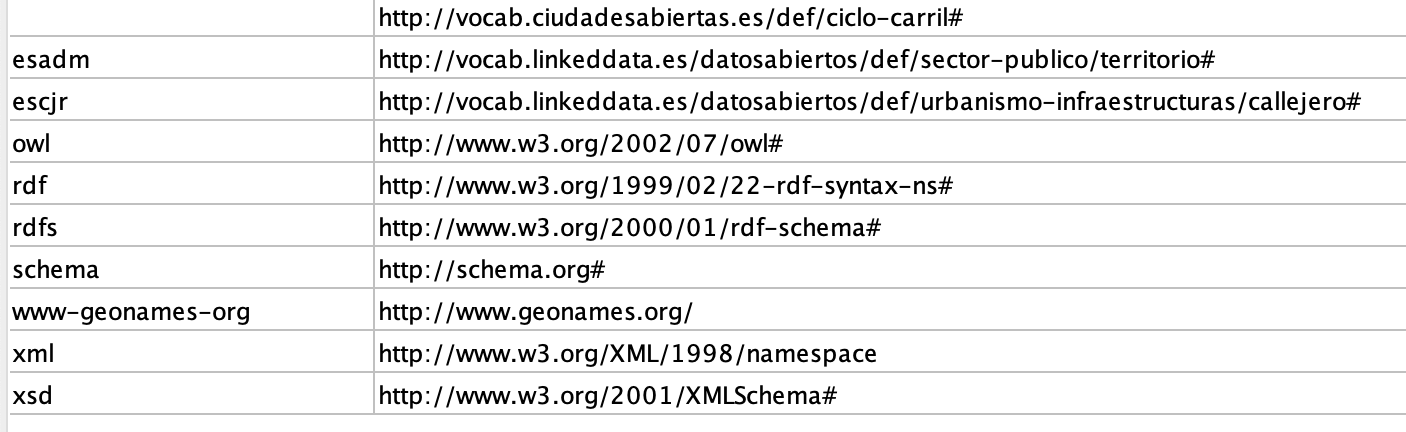
\includegraphics[angle=0, width=0.8\textwidth]{images/tablaIRIsCiclocarril.png}  
	\caption{Namespaces usados para Ciclocarriles}
\end{figure}




Cabe destacar en este conjunto de datos la ausencia de la propiedad TipoVia, presente en los demás utilizados. En este caso los nombres de las calles contenían únicamente palabras clave y privaban de la capacidad de obtener este atributo. En cambio si dispone de tipoUso, propiedad que indica si es una calle peatonal o ciclocarril.


Debido a la falta de disponibilidad de una leyenda o información proporcionada por el ayuntameinto de Madrid, para este conjunto de datos no se han podido conocer con exactitud el significado de sus datos. Se ha obtenido de forma aproximada esa información pero podria no ser correcta.


% En este caso la fecha no aporta nada por tanto no se pone...



